
\subsection{シミュレーション実験の目的}
直進動作のシミュレーション実験によって,脚軌道生成の失敗を防ぐためには,最小半径を140mmとすることが有効であるとわかった.
しかし,最小半径を140mmに設定すると,近似された脚の可動範囲が小さくなる.
そのため,先行研究の手法で歩行することができた地形であっても,歩行することができなくなる可能性がある.
直進動作時については,歩行することができることが確認できたため,
本章では,旋回動作を行う際に,最小半径を140mmとした場合に,歩行することができるかを検証することを目的とする.

先行研究では旋回動作は2次元空間でのみ実装されていたが,新たに3次元空間での旋回動作を実装したため,
先行研究で確認された地形を含めた3次元空間での旋回動作をシミュレーションで検証する.

\subsection{シミュレーション実験の条件}
シミュレーションを行うソフトウェア,シミュレーションを行う計算環境,
モデルとするロボットは直進動作のシミュレーション実験と同様であるため説明を省略する.
歩行条件についても直進動作のシミュレーション実験と同様とするが,
最小半径を140mmとし,動作は旋回動作とする.また,旋回は超信地旋回的に行う.

\subsubsection{歩行する地形}
先行研究でシミュレーションが行われた地形は,平地,亀裂のある地形,溝のある地形であるため,
これらの3つの地形でシミュレーションを行うこととした.
また,3次元空間での旋回動作を行うために,
これらの地形の中央に100mm,110mm,120mm,130mmの段差を設けた地形もシミュレーションに用いた.
さらに,これらの地形の全体を5度,10度,15度傾斜させた地形もシミュレーションに用いた.
段差を100mmから130mmとした理由は,波東らの研究によって,胴体姿勢を変更しない場合には上ることができる段差の高さの最大値が130mm程度であることがわかったためである.
傾斜を5度から15度とした理由も同様である.

\newpage

\begin{figure}[htbp]
  \begin{tabular}{cc}
    \begin{minipage}[t]{0.41\hsize}
      \begin{center}
      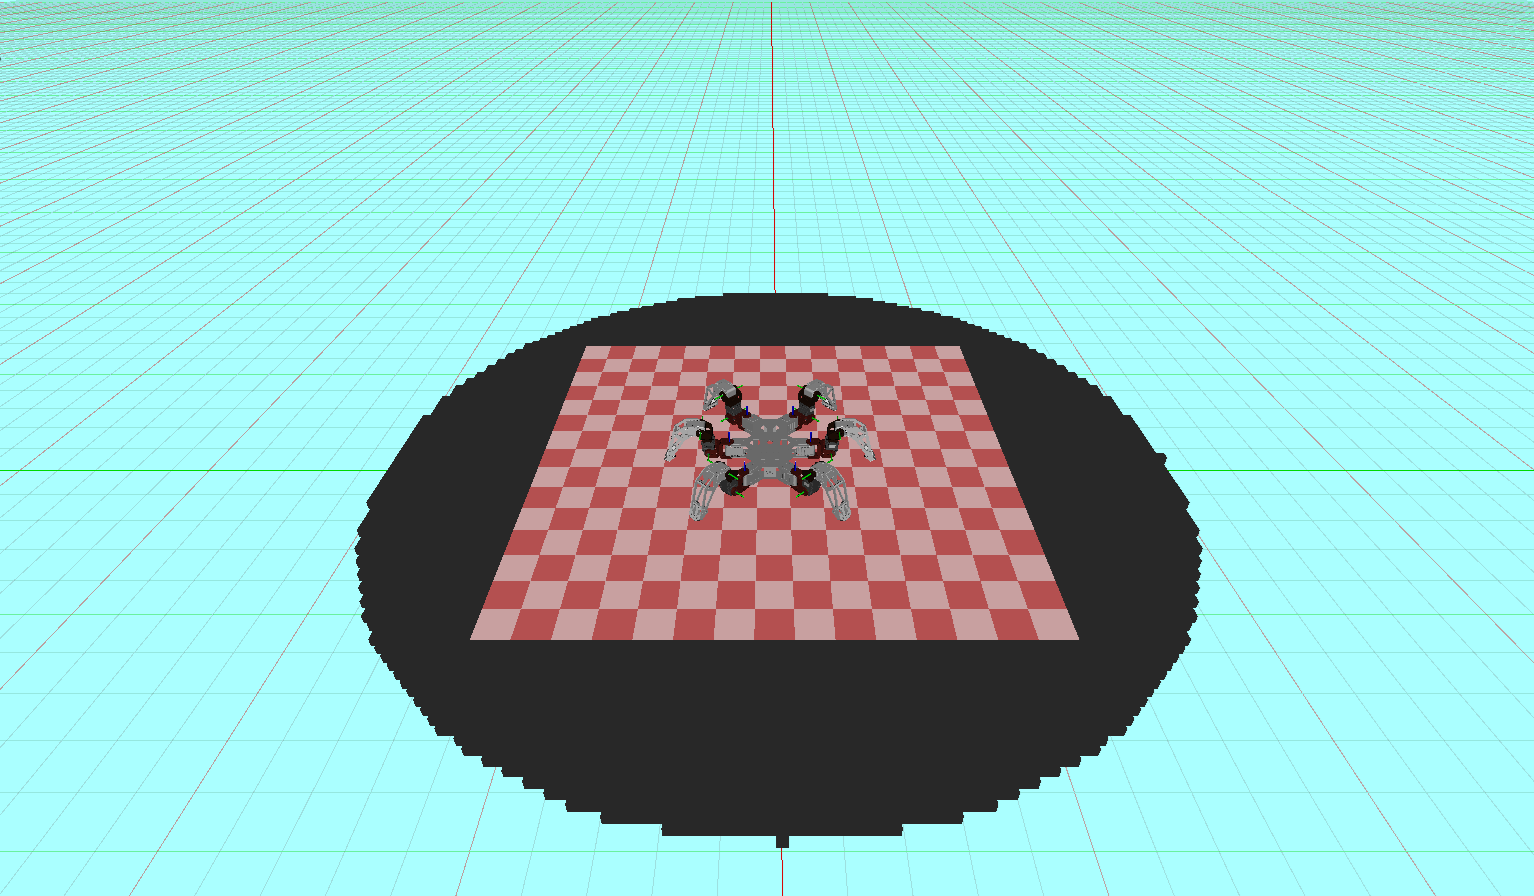
\includegraphics[width=1.0\linewidth,trim={30 30 30 30}, clip]{figure/chapter4/circle_flat.png}
      \text{(a) flat terrain}
      \end{center}
    \end{minipage} 
    &
    \begin{minipage}[t]{0.41\hsize}
      \begin{center}
      \includegraphics[width=1.0\linewidth,trim={30 30 30 30}, clip]{figure/chapter4/140mm/130mm.png}
      \text{(b) up step terrain}
      \end{center}  
    \end{minipage}
    \\
    \begin{minipage}[t]{0.41\hsize}
      \centering
      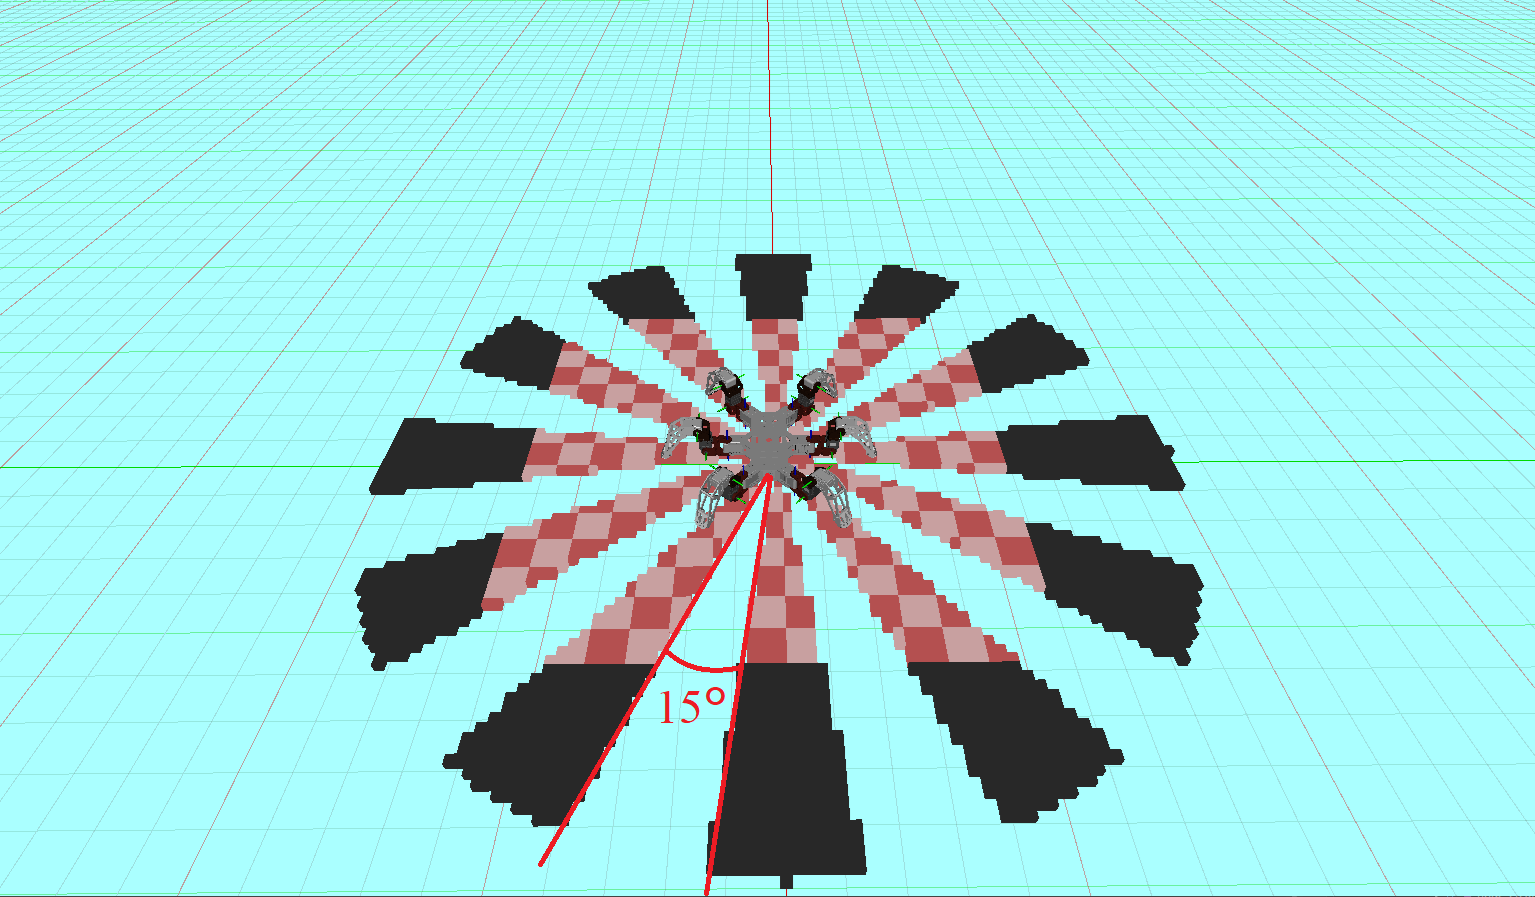
\includegraphics[width=1.0\linewidth,trim={30 30 30 30}, clip]{figure/chapter4/ditch.png}
      \centering
      \text{(c) ditched terrain}
    \end{minipage} 
    &    
    \\
  \end{tabular}
  \caption{Simulation Terrain}
  \label{fig:ch5_simu_terrain_turn} % chktex 24
\end{figure}

\subsubsection{シミュレーションの手順}
シミュレーションは次に示す手順で行った.
なお,旋回方向は時計回り,反時計回りの2つの方向でそれぞれシミュレーションを行った.
\begin{enumerate}
  \item ロボットの重心を地形から130mm離れるようにロボットを配置し,脚先は地形に接触している状態となるようにする.
  \item 旋回動作を行い,胴体が重力方向を軸として360度旋回するまでの歩容パターンを生成する.
  \item 歩容パターン生成に失敗することなく,また脚軌道生成に失敗することなく,360度旋回することができた場合を成功とする.
  \item 地形を変更し,(1)から(3)を繰り返す.各地形において旋回動作が成功するかを確認する.
\end{enumerate}



\subsection{シミュレーション実験の結果}

\subsection{考察}

結論として,最小半径を140mmとした場合でも,旋回動作を行うことができることがわかった.